\documentclass{IEEEtran} 
\usepackage{graphicx}
\usepackage{geometry}
\usepackage{amsmath}
\usepackage{amssymb}
\usepackage{multicol}
\usepackage{float}
\usepackage{booktabs}
\usepackage{changepage}
\usepackage{color}
\usepackage{longtable}

\geometry{top = 1 in, bottom = 1 in, right = 1 in, left = 1 in} 
\pagenumbering{gobble}
\title{Generating Random Numbers with Network Data}
\author{Micah A. Thornton, Neha N., Q. Zeng}
\date{\today}

\newtheorem{theorem}{Theorem}[section]
\newtheorem{lemma}[theorem]{Lemma}
\newtheorem{proposition}[theorem]{Proposition}
\newtheorem{corollary}[theorem]{Corollary}

\newenvironment{proof}[1][Proof]{\begin{trivlist}
\item[\hskip \labelsep {\bfseries #1}]}{\end{trivlist}}
\newenvironment{definition}[1][Definition]{\begin{trivlist}
\item[\hskip \labelsep {\bfseries #1}]}{\end{trivlist}}
\newenvironment{example}[1][Example]{\begin{trivlist}
\item[\hskip \labelsep {\bfseries #1}]}{\end{trivlist}}
\newenvironment{remark}[1][Remark]{\begin{trivlist}
\item[\hskip \labelsep {\bfseries #1}]}{\end{trivlist}}

\newcommand{\qed}{\nobreak \ifvmode \relax \else
      \ifdim\lastskip<1.5em \hskip-\lastskip
      \hskip1.5em plus0em minus0.5em \fi \nobreak
      \vrule height0.75em width0.5em depth0.25em\fi}



\begin{document}
\maketitle{}

\begin{abstract}

\end{abstract} 

\section{Introduction} 
A  true random number is a range of possible value usually drawn statistically. Random values  are used utilized by many applications, from OS-level functionality for stack pointer randomization, facilitating gaming, scientific computing and for computer security for cryptographic key generation.{new citations}A true random number generator uses a physical phenomenon as a source for the generation of randomness like a little variation in the movement of your mouse or keystroke. On the other hand the pseudo random number generator uses algorithms, mathematical formulae or a precalculated table as source for the generation of randomness.Random.org is one of the example of true random number generator while linear congruential generator is of pseudo random number generator.  
Out of the many sources possible for the generation of random numbers,  Linux being one of them due to its inbuilt PRNG,  one of the major drawback  would  be the  system running out entropy i.e a drop in the  level of entropy.  The linux system uses /dev/random and /dev/urandom for the generation of random numbers and both the interfaces behave differently in case of low entropy level. The dev/random blocks until the entropy level is high thus leading to delays and degrading the quality of services while the /dev/urandom does not block but the random data may not be suited for security related applications. Also the source of random number generator on linux is limited and may not be suitable for generation of large amount of random data.  
In this paper huge amount of  random number were generated in linux, with the help of the network data. The entropy was processed using the network data that was captured instead of using the entropy of the operating system. This technique could be used as an additional source of Random Number Generator when a higher quantity of random numbers are needed for applications such as computer security. This is a feasible technique as every computer now-a-days comes equipped with a network Interface Card and the network data could prove to be a good source of random values.We  also  further analyzed the change in the sequence in case of an known attack that may have occurred on the network with the help of NIST test.



\section{Related Work}

There has been a substantial amount of work on the generation of random numbers using modern devices such as cellular automata, and Multiple-mersenne twisters [CITATION NEEDED]. As well as the use of natural phenomenon to generate random numbers, some such techniques are discussed here. \cite{Mul13} 

\subsection{PRNG Linux system}

Linux is one of the most popular operating system used in the world which serves as an operating system for a variety of applications and it provides a built in service for the generation of random numbers. The  Linux RNG uses the kernel space for the generation of Random Numbers. It  consist of three components, first which converts events into bits and is the  key source for entropy. The second component is responsible for the addition of these bits to the generator pools and the third component applies three consecutive  SHA-1 operations when the bits are read from the generator which in turn generates the output of the generator which is then feed back into the pool. The randomness generated is received in the form of a word i.e 32 bits. An account  of the amount of physical randomness added into the pool is done with the help of counter which is calculated as a function of the different system events occurring. This counter value is denoted as entropy in case of Linux Random Number Generator.

 
\subsection{Kernel level random number generator}

Linux has a kernel-level random number generator and is abstracted as a 2-character device /dev/random and /dev/urandom. The former is a blocking random number generator, the latter is a non-blocking random number generator. \cite{Vui12, Gut06, Vie03}

\subsubsection{Blocked random number generator}

The application can read the random number values in the /dev/random internal entropy pool through the read () system call. The read () system call is blocked when the number of random numbers in the entropy pool is less than the number of applications to read, the application is suspended.

\subsubsection{Non-blocking random number generator}

/dev/urandom is a non-blocking pseudo-random number generating program that can be supplied to any number of random numbers of the application at any time. When the application requires too many random numbers, the entropy pool cannot be updated in time, so its entropy will be reduced. Same with /dev/urandom, the application reads through the read () system call random number value.
Qualitative Analysis of Kernel Level Random Number Generator Performance

The application must call the read () system call to get the random number from /dev/random or /dev/urandom, and the read () system call will cause the system context to switch. Visible, from the application's perspective, the random number generated delay includes not only the delay of the random number algorithm itself, but also the overhead of context switching, etc. For network security applications where the key translation is frequent, if the delay generated by the random number is large, the performance of the application will be degraded. Obviously, this is unacceptable for such applications.

\subsection{Random Number Sources}

In order to facilitate software debugging and performance measurements, Intel has built a timestamp counter in its Pentium processor and subsequent processors (TSC, Time Stamp Counter). TSC is a 64 bit hardware counter with a count of one for each processor clock cycle.  Application can be non-privileged instructions RDTSC read TSC count value. Fast algorithm using TSC as a random number. Since the application can access TSC directly in user space, this allows fast algorithms to be implemented in user space.

SHA is widely used in cryptographic algorithms, key hash validation and the generation of random numbers. SHA cannot infer the input of SHA because of the irreversibility of the one-way hash function that cannot be based on the input of the existing random number inverse algorithm Subsequent random numbers, so the random number generated by SHA is unpredictable, ensuring that the generated random number is safe.


\subsection{Mobile and IOT Devices}

Random Number in Android is based on the Linux Random Number Generator. APRNG mainly consist of two parts the Entropy Mixer  which is used to preserve the current state of /dev/urandom  and the Secure Random Front end acts as current SHA1PRNG which is a current provider for cryptographically secure random numbers for Android OS. Initial algorithms proposed for the generation of randomness and which is currently being utilized for IOS is the Yarrow RNG. Intel uses RDRAND instruction for entropy generation or for generation of random number The Intel Data Protection Technology is accessible through RDRAND and RDSEED which provide a wide range of statistical random numbers which do not require any additional libraries or operating system handling.

 A more novel Sensor based approach for IOT and Mobile device is developed which uses noise in the sensor data as a source of Random number generator  which produces a less computational overhead in comparison to the current Android Pseudo Random Generator. \cite{Wal16}

\subsection{Virtual Machine}

The paper about Not-So-Random Numbers in Virtualized Linux and the Whirlwind RNG by Yan Zhai mentions about how Linux operating system generates and how they attempt to harvest entropy form various hardware sources. A new Whirlwind approach is specified for generating secure  randomness which is developed with a view to rectify the current problem with the existing VM reset vulnerabilities which reuses the internal state to develop random number which may not be very secure when used for  cryptographic applications. \cite{Fer13}


\section{Harvesting Entropy}
Although sources of entropy are frequently gathered by modern random number generators, there is not much information on how the harvested entropy foments useful random numbers. As was stated in the introduction the Linux random number generator does extract entropy from interrupts, disk accesses, keyboard input, and more, but not much is said on how the entropy is actually taken from these events. 

One obvious metric to examine when attempting to extract entropy timing. For instance, when harvesting entropy from the keyboard, one possible method for doing so is the careful examination of the wait times between key presses. The slight variations in key presses may not be a \textit{truly} random data source (I.e. the distribution may not be uniform), but there are many methods for transforming known distributions into uniform ones, one such method is the first of, what we claim, are three ways to harvest entropy from a random stream. 

\subsection{A Posteriori Coin-Flip}

The principle behind this method of entropy harvesting relies on a known data set size. After the data is collected, the median value of the distribution is calculated. Since by definition the median is a measure of center, calculated as the middle element of the data set, exactly one half of the retrieved values will be above the median and the other will be below. Obviously, this extends to the use of other measures of center, and even potentially trend models such as a Linear regression, ARMA and other forecasting techniques. 

The A Posteriori Coin-Flip occurs after your entire data set has been collected and a valid trend seeking line (whether flat as with the mean or median, or sloped), begin at the first data point (this is the first coin-flip) if it lies above the calculated measure of center (MOC) record one, or heads as the result of the first coin-flip. Continue until all data points have been assigned a bit. This bitstring is an example of extracting entropy from a system if you are given knowledge about the data system ahead of time. Mathematically this notion can be expressed in the following way. 

\begin{definition} \textbf{1 A Posteriori Coin-Flip} \\
\begin{center}
Given $X$ such that $X=\{x_1,x_2,x_3,...,x_n\}$ \\
\end{center}
$$Q_2 = \{x|P(X>x)=P(X<x)=0.5\}$$
$$R_\psi(x_i) = r_i = \begin{cases} 
      1 & x_i > Q_2 \\
      0 & x_i < Q_2
   \end{cases}$$
\begin{center}
Hence, the entropy is extracted into the binary value: $r_1r_2r_3r_4...r_n$
\end{center}
\end{definition}

In this definition we are using the median as the MOC (represented by $Q_2$), however this can easily be replaced with any other MOC. As with any method there is a short pros and cons list for using the A Posteriori Coin-Flip. One obvious con of the definition in the manner we present it with a static MOC, as opposed to a dynamic MOC such as a time series ARMA model, there will tend to be an obvious correlation between values close together. Of course, the better the entropy source, the higher quality the harvested entropy will be. A Pro of using this method is that we can force a uniform distribution on the output string. A further benefit of using this method is that the MOC must only be calculated one time (after all of the data is collected) 

A mathematical proof that this method (using the median) will harvest the maximum theoretical entropy is given here: 

\begin{proof} \textbf{A Posteriori Coin-Flip maximizes Shannon Entropy} \\
Given a \textit{supposedly} random sample $$X = \{x_1 \in \mathbb{R},x_2\in \mathbb{R},x_3\in \mathbb{R},...,x_n\in \mathbb{R}\}$$We define the random variable $\alpha$ in terms of the median (or second quartile) of $X$ $$\alpha:\mathbb{R}\to\mathbb{B}$$ $$P(\alpha =  0) = p_0(\alpha) = \frac{\vert\{x\vert x<Q_2(X)\}\vert}{\vert X \vert} = \frac{1}{2} $$ $$P(\alpha =  1) = p_1(\alpha) = \frac{\vert\{x\vert x>Q_2(X)\}\vert}{\vert X \vert} = \frac{1}{2}$$The formula for the entropy of a string of Bernoulli trials (or a `bitstring') is given:$$H(p_0(b),p_1(b)) = -(p_0(b)\textrm{log}_2(p_0(b)) +p_1(b)\textrm{log}_2(p_1(b)))$$ We can maximize the Entropy function as so:$$\nabla H(p_0,p_1) = \Big(\frac{\partial H}{\partial p_0},\frac{\partial H}{\partial p_1}\Big) = \Big(-\frac{\textrm{ln}(p_0) + 1}{\textrm{ln}(2)},-\frac{\textrm{ln}(p_1) + 1}{\textrm{ln}(2)}\Big)$$Maximizing we find$$\frac{-\textrm{ln}(p_0) - 1}{\textrm{ln}(2)} = 0 \implies \textrm{ln}(p_0) = -1 \implies p_0 = \frac{1}{e}$$ $$\frac{-\textrm{ln}(p_1) - 1}{\textrm{ln}(2)} = 0 \implies \textrm{ln}(p_1) = -1 \implies p_1 = \frac{1}{e}$$This seemingly odd result is because there is an \textit{inherent} dependence among these two values, expressed mathematically as $p_0 + p_1 = 1$, in our first maximization attempt, we neglected to account for the hard-restraint $p_0 +p_1 = 1$ In constraining the original optimization we have the following system: 
$$\frac{-\textrm{ln}(p_1) - 1}{\textrm{ln}(2)} = 0 = \frac{-\textrm{ln}(p_0) - 1}{\textrm{ln}(2)}$$
$$ p_1 = 1-p_0$$
$$ \frac{-\textrm{ln}(1-p_0) - 1}{\textrm{ln}(2)} = \frac{-\textrm{ln}(p_0) - 1}{\textrm{ln}(2)} \implies 1-p_0 = p_0$$$$ \implies p_0 = 0.5 \implies p_1 = 1 - 0.5 = 0.5$$Because $p_0(\alpha) = p_1(\alpha) = 0.5$ by definition, we have maximized the entropy function for the constraint $p_1 + p_0 = 1$.\hfill  $\qed$
\end{proof}

\begin{corollary}
The author would like to note that the characterization of the bias in this formula is potentially a novel concept, and suggests that a more natural measurement of entropy extends by adding the factor $(\frac{1}{2} - \frac{1}{e})$ to the probabilities $p_0$ and $p_1$ before using the original definition of the formula. (this will increase the maximum possible entropy in a string to $\frac{2}{e \cdot \textrm{log(2)}}$ but it can be rescaled accordingly using simple ratios)
\end{corollary}

\subsection{Extemporaneous Coin-Flip}

As the name implies, the extemporaneous coin-flip occurs simultaneously as new data is available. The general procedure is very similar to that of the A Posteriori coin-flip, however in this method the measure of center is recomputed with every new sample that becomes available. In this method we start with an initial guess as to the measure of center (This could be a MOC from a previous entropy capture, or an educated guess, or simply the first value observed). As a side note, in both this and the A Priori Coin-Flip method, the first random bit retrieved can and should be thrown away in certain circumstances. 

As with the previous method, each time new data becomes available it is compared to the MOC and a bit is generated depending on whether the point lies above or below. Unlike the previous example, the MOC changes with every new data point available. in the following definition the chosen MOC is again the median, however again this can easily be replaced with whichever statistic is desired. 

\begin{definition} \textbf{2 Extemporaneous Coin-Flip} \\

\begin{center}
Given a series of sets $X = \{X_1,X_2,X_3,...,X_n\}$ \\ 
Such that $X_1 \subset X_2 \subset X_3 \subset ... \subset X_n$ \\ 
$\{ \forall i \in \mathbb{N} \vert 0 < i \leq n\} \implies \vert X_i\vert + 1 = \vert X_{i-1} \vert $ \\

\end{center} Given an initial guess $g_0$ to serve as the MOC (before the first data point is collected) We can express our updating median as a function of data sets in the following manner.

$$Q_2(X_i) = \{x|P(X_i > x) = P(X_i < x) = 0.5\}$$ 
$$R_\phi(x_i) =  r_i = \begin{cases} 
      1 & x_i > Q_2(X_i) \\
      0 & x_i < Q_2(X_i)
   \end{cases}$$

As with the previous definition the entropy generated can be utilized by the bitstream given by: 

$$r_1r_2r_3r_4...r_n$$
\end{definition} 

As with the A Posteriori method, there are some benefits, and draw backs to using this method for entropy extraction. In this method the measure of center must be recomputed with each subsequent data point gathered, this could waste valuable CPU cycles. The primary benefit of using this method is that after the new MOC is calculated, the old can be discarded, as well as the immediate discarding of all previous data, as it is analyzed simultaneously as it is gathered. This method is also easy to implement on systems where you would like to be constantly analyzing data (such as massive server banks connected to Muller-Geiger tubes and old fire detector parts). 

\subsection{A Priori Coin-Flip}

The last of what we claim are three entropy extraction methodologies presented in this work we again require some guess or `A priori' knowledge in order to effectively use the first bit as a truly random coin flip. This method is performed in exactly the same manner as the previous, with one key difference. In this method, the MOC that is used must determine the outcome of the coin-flip \textbf{before} it is updated with the new information. The new value must be used to update the MOC after the previous coin-flip, both the previous data value and previous MOC can be immediately discarded after the new MOC is generated. As it is essentially the same method as above simply time-lagged by one observation the definition is very similar with the difference highlighted below

\begin{definition}
\textbf{3 A Priori Coin-Flip} \\ 
\begin{center}
Given a series of sets $X = \{X_1,X_2,X_3,...,X_n\}$ \\ 
Such that $X_1 \subset X_2 \subset X_3 \subset ... \subset X_n$ \\ 
$\{ \forall i \in \mathbb{N} \vert 0 \leq i \leq n\} \implies \vert X_i\vert + 1 = \vert X_{i-1} \vert $ \\

\end{center} Given an initial guess $g_0$ to serve as the MOC (before the first data point is collected) We can express our updating median as a function of data sets in the following manner.

$$Q_2(X_i) = \begin{cases} 
      \{x|P(X_i > x) = P(X_i < x) = 0.5\} & i \neq 1 \\
      g_0 & i = 0
      \end{cases}$$ 
$$R_\pi(x_i) =  r_i = \begin{cases} 
      1 & x_i > Q_2(X_{i-1}) \\
      0 & x_i < Q_2(X_{i-1})
   \end{cases}$$

The entropy is in the bit string: 

$$r_1r_2r_3r_4...r_n$$
\end{definition} 

\begin{corollary} 
This method can easily be extended ad inf. by using MOC's from more than one observation in the past, then updating with a lag value greater than one. 
\end{corollary}

\begin{corollary}
When using certain methods for the MOC, such as forecasting models for time series, prior data must be kept for the recalculation of the MOC, however, a sliding window could also be used in this case to save memory. \\ 
\end{corollary}
Many of the pros and cons for using this method correspond with what was said about the Extemporaneous Coin-Flip. In this method, unlike the last, the new MOC does not need to be calculated before the result of the next coin-flip can be determined. This is a great method to use when events are rare, and there is a long wait time before the next observation. When using this method in the given scenario, the wait time can be used as compute time for the updated MOC. 

It is essential to note that in all of the above methods the entropy extracted from the random stream should not be used directly (I.e. do not directly use the bit strings calculated as your random values), they should instead be used as inputs to pseudo-random number generators, conglomerated with multiple other sources of entropy with a mixing function, or as we will further explore in this work use pseudo-random functions such as cryptographic primitives like hash functions and HMACs (potentially even using the random value a key in a keyed HMAC). One could even potentially use a good compression algorithm to produce a valuable random number. 

%\section{Case Study: Packet Capture Entropy Harvest}
\section{Harvesting Entropy from Network Timing Data} 
In this section we attempt to harvest entropy from an real-life random stream, that almost any modern computer has access to. We propose the harvesting of entropy from simple packet capture data. This notion extends much further than the manner in which it is presented here, and can be applied to far more sophisticated broadcast data (I.e. low band AM, Snow on television). In this case, we take a very clearly deliberate and logical approach to extracting entropy. 

We briefly mentioned in the last section that a straightforward approach to extracting entropy from a random stream is to investigate the timings of the events. In this specific application we examine the timing data for packets using a standard packet capture tool (Wireshark). Once a given packet capture was completed we computed the retrieved entropy bit strings using the A Posteriori method described in the previous section. 

With our packet capture results, timing data was given in terms of seconds (with 5 digits of significance). As each time was initially reported in the elapsed time since the beginning of the capture, we first needed to subtract each next arrival time from the prior arrival time. In this manner each of the packets received would be assigned a time delta, (or in other words, the time stamp of the packet received after the current packet minus the current packet's time stamp. We can formally define this in the following manner. 

\begin{definition}
\textbf{4 Harvesting Entropy from Packet Timing Data} \\
let $t_i$ represent the $i^{th}$ time stamp given in seconds, since the beginning of the packet capture. 
$$\delta_i = t_{i+1} - t_{i}$$
Note that this necessarily excludes the generation of the terminal $\delta_i$ (because $t_{i+1}$ has not been observed yet). Suppose that in a given packet capture, $n$ packets are captured, then
$$\Delta = \{\delta_1,\delta_2,..,\delta_{n-1}\}$$
We can then define a probability space over the set $\Delta$
$$P(\overline{\Delta} < x) =  \frac{\vert\{\delta_i \in \Delta| \delta_i < x\}\vert}{\vert \Delta \vert}$$
$$Q_2 = \{\delta \vert P(\overline{\Delta} < \delta) = P(\overline{\Delta} > \delta) = 0.5\}$$
We then simply perform the A Posteriori Coin-Flip discussed in the previous section
$$R_\psi(\delta_i) =  r_i = \begin{cases} 
      1 & \delta_i > Q_2 \\
      0 & \delta_i < Q_2
   \end{cases}$$

\end{definition}

\section{Results} 

Packet captures of sizes ranging from 5000-50000 packets were run at three different times, and over multiple networks on three different operating systems (Mac OSX, Windows 10, Ubuntu Linux 16.10). 

\begin{figure}[H]
\caption{Packet Timings in Various OS}
\begin{center}
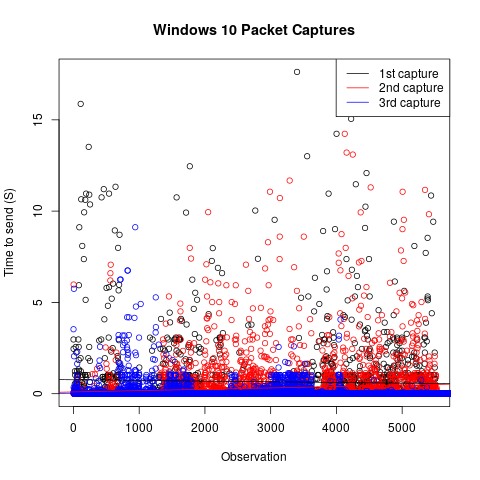
\includegraphics[scale=0.3]{../Neha2.png}
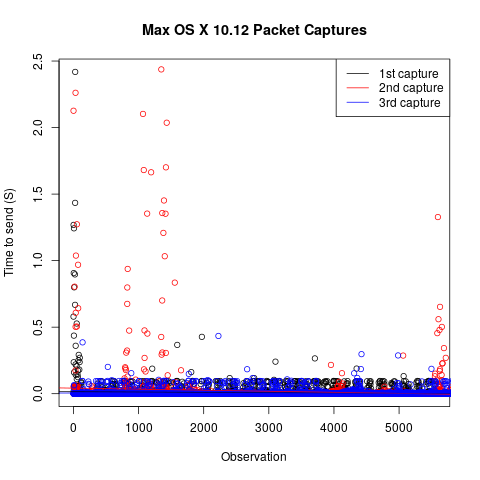
\includegraphics[scale=0.3]{../Zeng2.png}
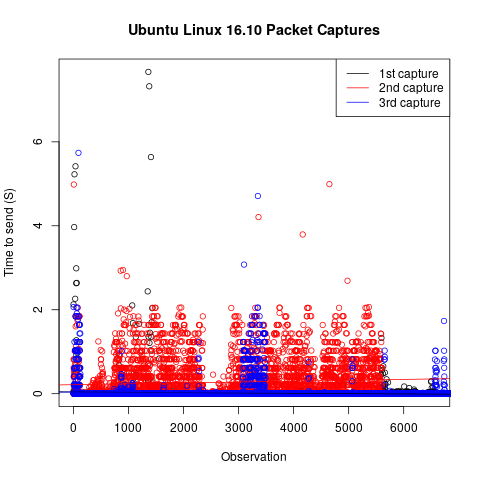
\includegraphics[scale=0.3]{../Micah2.png}
\end{center}

\end{figure}

A very quick inspection of the plots reveals that there is  temporal correlation in the data at this point, however, we are not worried about the quality of the random numbers produced at this stage in their creation. As was stated in Section III, we are not going to simply use the produced value, we are more likely to use the gathered entropy to seed a deterministic pseudorandom generator. 

We leave it to future work to perform more sophisticated trend modeling, in this analysis we will simply be using the median to decide the outcome of the A Posteriori Coin-Flip. The medians were calculated and nine different entropic bit strings were collected. 

\section{Analysis}
In our analysis we will simply be using the Linux utility ENT, created at Fourmilabs, which reports several statistics on the entropy contained, temporal correlations, even quality of randomness (Monte Carlo simulation of Pi). In the following paragraphs we will briefly examine and discuss the use of each of the statistics that are calculated using ENT, as well as presenting a table of the results for the entropic strings that were generated using the A Posteriori Coin-Flip method on our nine packet capture timing Data vectors. 

The first metric reported by ENT is its name-sake: entropy. For all intents and purposes we can think of this measure as a rough estimate as to how much information is actually contained within a bitstring. The metric of entropy was defined by Claude Shannon in his seminal work \textit{A Mathematical Theory of Communication}. The formula he gives for approximating the entropy of a bit string is defined as: 

\begin{definition}
\textbf{Shannon Entropy (as applied to bitstrings)} \\
The Shannon Entropy of a bitstring is quantified in terms of the information inherently contained by the string. The derivation of this formula is very simple and intuitive. Shannon entropy is defined as: 

$$H(X) = -\sum_{i=1}^n{p_i \textrm{log}_2(p_i)} $$

In a bitstring, there are two possible outcomes, either a one or a zero. Hence there are only two probabilities to deal with, $p_0 = P(\overline{X} = 0)$ and $p_1 = P(\overline{X} = 1)$ for random variable $\overline{X}$, which is distributed according to the relative frequency distribution for bits contained within the random string $X = x_1x_2x_3..x_n$. In this way, the entropy is calculated in a very similar manner to that of the way which it is extracted in the A Posteriori Coin-Flip, where we must have retrieved all information before we can provide an accurate estimate. Once we have collected all of the data, and calculated $\{p_0,p_1\}$ we can calculate the entropy of the bit string directly as: 

$$H(X) = -[p_1\textrm{log}_2(p_1) + p_0\textrm{log}_2(p_0)]$$
\end{definition}

\begin{corollary}
The authors suggest the use of an iterative distribution update, or prior distribution update when harvesting random data from a continuous string. In the same manner as the iteratively updating MOC in the Extemporaneous, and A Priori Coin-Flip methods. 
\end{corollary}

The entropy is reported in terms of a measurement of the amount of `bits' of information contained in a specific character, in the case of a random bit string it reports the `bits' per bit. Hence in the \textit{ideal} case we would see entropy approaching 1.0 (or subsequently, the number of bits used to encode the symbol)


The second statistic reported on by ENT is the optimum compression ratio. Note that, this is calculated directly from the entropy estimate. We also would like to note that because of this, it may not take more useful and modern compression techniques into account and is simply a theoretical value. The statistic is reported in relation to compression on bytes, as well as the compression for the value as a bit string. Again, thanks to Claude Shannon, a theoretical maximum value for the optimum compression ratio was quantized in terms of the entropy of the string to be compressed. 

\begin{definition}
\textbf{Shannon's Source Coding Theorem} \\
This theorem simply states that the length of the optimally compressed string is directly related to the entropy contained over the entire string, Note that this is not the ratio of entropy per symbol as it is reported by ent, it is technically equivalent to the entropy ratio reported by ent multiplied by the length of the string in symbols. Mathematically the bound on the minimum length of a compressed string is given as: 

$$L_c < H(X) + \frac{1}{N}$$

Where $L_c$ is the minimum length of the compressed string $X$ of length $N$. The Compression ratio then simply becomes: 

$$C= \frac{L_u - L_c}{L_u}$$
\end{definition}
Where $L_u$ and $L_c$ are the uncompressed and compressed string lengths. Ideally, the entropy ratio is close to one bit per bit, and therefore there the difference $L_u-L_c$ will approach zero, causing the compression ratio to become zero. The theoretical nature of this calculation does not apply to different compression methods, such as run-length encoding. 

The next statistical result reported on by ent are the results of a chi-squared($\chi^2$) test for randomness. The $\chi^2$-test was first proposed by Karl Pearson, an extremely prolific statistician out of London England. As with any statistical hypothesis test this test is formulated by examining collected data through the use of a deterministic function of said data known as a statistic. The statistic, or test-statistic, is then compared to a critical point on the \textbf{Known Distribution} of test-statistics to ascertain whether or not a specific hypothesis should be rejected. In this way, it is similar to the Coin-Flip methods described above, however the MOC would correspond to the critical-value on the distribution of test-statistics. The key contribution of Pearson to this particular test was his proof that a test statistic (deterministic function of the data) would be distributed (in the theoretical case) according to a parameterized distribution known as the $\chi^2$ distribution (so named as the square of the sum of normally distributed random variables follows this distribution). The $\chi^2$ distribution is a parameterized distribution, meaning that the deterministic function providing its probability density function (PDF) is dependent on a value supplied in the instantiation of the distribution. The required value for the $\chi^2$ distribution is given the symbol $\kappa$ and known as the ``degrees of freedom''. Degrees of freedom are so called, because when special conditions are met, they can be calculated indirectly as a function of how much data was collected, however it should be noted that this is simply an estimate, as was proven in Kendall's Advanced theory of Statistics.

In the case of the $\chi^2$ test, it was shown that the sum of the squared differences in frequencies between that of an observed distribution, and that of a theoretical distribution divided by the theoretical distribution, for each discretized observation bin will follow a $\chi^2$ distribution with degrees of freedom calculated by use of the number of observation bins $n$, and the number of co-variates used to specify the theoretical distribution $p$. Again due to Shannon, it was speculated that if data were to be truly random, it would be pulled from a Uniform distribution, with two parameters (a which is the first observation,b which is the last observation). Therefore, to use the proposed test for randomness, the theoretical distribution that will be used is the uniform distribution. Hence a $\chi^2$ test for randomness can be mathematically formulated in the following way: 

\begin{definition}
\textbf{Chi-Square test for Randomness} \\
Given a set of \textbf{discrete} observations $X = {x_1,x_2,x_3,...,x_n}$, we wish to show: 
$$(\overline{X}:X \to X)\sim U[x_1,x_n]$$ 

\textit{The random variable $\overline{X}$ defined as a mapping of data points to themselves in the measure space is distributed sufficiently close to, or far away from the given uniform distribution. }

$$H_0: \overline{X} \sim U[x_1,x_n]$$
$$H_1: \overline{X} \sim \Lambda$$ 

Where $\Lambda$ is an unknown distribution. A significance level $\alpha$, denoting the point of the critical value (I.e. which determines \textit{how similar} the frequencies must be to \textbf{not reject the null hypothesis}) is chosen. A standard value is $\alpha = 0.05$. Calculating the test statistic, and determining the critical point on the appropriate $\chi^2$ distribution as shown here: 

$$c_p = \{x \vert P(\chi^2(\kappa) < x) = \alpha = 0.05\}$$
$$\chi^2 = \sum_{i=1}^n{\frac{(O_i - T_i)^2}{T_i}}$$
$$\kappa = n - (p+1)$$ 

Note that the definition of how many bins exist depends strongly on the manner in which a random string is analyzed. In ent, for instance, when running in byte mode, there are $2^8 = 256$ bins, whereas when analyzing in bit mode, there are only two bins, one and zero. 
\end{definition}

\begin{remark}
The ent results also report the tail probability (`it will exceed this value less than X percent of the time'). This value is also known as the p-value, if the p-value is greater than our significance level $\alpha$ then we fail to reject the possibility that the data does indeed come from a random distribution.
\end{remark}

Fourmilabs, the creator of ent, suggests the following interpretations for $\chi^2$ test results. 


\begin{table}[h!]
\centering
\caption{$\chi^2$ p-value interpretations}
\begin{tabular}{|c|c|}
\hline
\textbf{p-value} & \textbf{Interpretation}\\
\hline
p-val $>$ 99\% & Almost certainly not random.\\
\hline
99\% $<$ p-val $>$ 95\% & The sequence is suspect.\\
\hline 
95\% $<$ p-val $>$ 90\% & The sequence is almost suspect.\\
\hline
90\% $<$ p-val $>$ 10\% & The sequence is good.\\
\hline
10\% $<$ p-val $>$ 5\% & The sequence is almost suspect.\\
\hline
5\% $<$ p-val $>$ 1\% & The sequence is suspect.\\ 
\hline 
p-val $<$ 1\% & Almost certainly not random.\\
\hline
\end{tabular}
\end{table}

The next parameter reported by ent is the arithmetic mean of the data, depending on whether you specify byte or bit mode in ent, this will produce an average of the binary numbers encoded in a single byte (0-255) or, simply the bits present in the file. It is calculated simply by summing every value, and dividing by the number of values present. We could further use the calculated mean as a test-statistic in a student's t-test, however it is sufficient to simply compare to the ideal means 0.5, and 127.5 for bits and bytes respectively.

In another test, the ent suite reports the monte-carlo simulation value for pi. 


\bibliographystyle{plain}
\bibliography{biblio}


\begin{table*}[h!]
\begin{adjustwidth}{-1.25 cm}{}
\centering
\caption{Pure Entropic String ENT results}
\begin{tabular}{@{}rrrrcrrrcrrrr@{}}\toprule
& \multicolumn{2}{c}{\textbf{Entropy}} & \phantom{abc}& \multicolumn{2}{c}{\textbf{Arithmetic Mean}} &
\phantom{abc} & \multicolumn{2}{c}{\textbf{Serial Correlation}} & \phantom{abc} &\multicolumn{3}{c}{\textbf{Compression}}\\
\cmidrule{2-3} \cmidrule{5-6} \cmidrule{8-9} \cmidrule{11-13}
& \textit{bits/byte} & \textit{bits/bit}  && \textit{by byte} & \textit{by bit} && \textit{by byte} & \textit{by bit} && \textit{size (b)} & \textit{comp. size (b)} & \textit{ratio (\%)}\\ \midrule
\textbf{Windows 10}\\
\textit{Capture 1} & 6.666783 & 0.999995  && 126.5384 & 0.4986  && -0.104782 & 0.207267 && 2200 & 2200 & 0\\
\textit{Capture 2}& 7.196086& 1.000000&& 125.5073& 0.4998&& 0.083004& 0.209302 && 5504 & 5504 & 0\\
\textit{Capture 3}& 7.362089& 1.000000&& 126.5384& 0.4997&& 0.374569& 0.232915 && 11472 & 11472 & 0\\
\textbf{Mac OS X 12.10}\\
\textit{Capture 1} & 7.198828 & 1.000000  && 125.7977 & 0.5000 && 0.326609 & 0.070809 && 5536 & 5536 & 0 \\
\textit{Capture 2}& 7.229747& 1.000000&& 126.3883& 0.5000&& 0.249999& 0.119658 && 6552 & 6552 & 0\\
\textit{Capture 3}& 3.843544& 0.980664&& 71.4336& 0.4183&& 0.397400&  0.018324 && 11680 & 11563 & 1 \\
\textbf{Ubuntu Linux 16.10}\\
\textit{Capture 1} & 7.229747 & 1.000000  && 126.3883 & 0.5000 && 0.249999 & 0.119658 && 6552 & 6552 & 0 \\
\textit{Capture 2}& 6.973394& 0.999999&& 127.8026& 0.4993&& 0.313810& 0.307581 && 5592 & 5592 &0\\
\textit{Capture 3}& 5.304753& 1.000000&& 128.1367& 0.5001&&-0.003104& 0.682508&& 50080 & 50080 & 0\\
\bottomrule
\textbf{Averages}\\
\textit{Linux}& 6.503 & 1.0 && 127.4 &0.4998  && 0.188971  & 0.3699 && - & - & 0\\
\textit{Mac}& 6.091 & 0.9936&& 107.87 &0.4728 && 0.3247 & 0.06960 && - & - & 0.3333\\
\textit{PC}& 7.075 & 1.0 && 126.2 &0.4994 && 0.11760 & 0.2165 && - & - & 0\\
\textbf{Reference}\\
\textit{Hotbits} & 7.916369 & 0.999995  && 128.7873 & 0.4987 && 0.031555 & 0.000973 && 16320 & 16320 & 0\\
\textit{Ideal}& 8.0& 1.0&& 127.5& 0.5&& 0.0& 0.0 && - & - & 0\\
\bottomrule
\textbf{Cross Platform Average}& 6.5563 & 0.997867 && 120.49 & 0.49067 && 0.21042367 &0.21867 && - & - & 10\\
\bottomrule
\end{tabular}
\end{adjustwidth}
\end{table*}



\newpage
\onecolumn

\begin{center}
\textsc{Table of Hashed Packet Data ENT results (by bits)}
\end{center}
\begin{longtable}{rllrrrrrr}
  \hline
 & Operating.System & Hash & Size & Entropy & Chi.Sq. & Mean & MC.Pi & Serial.Correlation \\ 
  \hline
1 & Linux & bl2b &    6656 & 0.999993 & 0.060096 & 0.498498 & 3.217391 & -0.013230 \\ 
  2 & Linux & bl2b &    5632 & 0.999960 & 0.313210 & 0.503729 & 3.247863 & -0.004317 \\ 
  3 & Linux & bl2b &   50176 & 0.999996 & 0.277503 & 0.498824 & 3.058373 & 0.004060 \\ 
  4 & Windows & bl2b &    2560 & 0.999901 & 0.351562 & 0.505859 & 3.396226 & 0.018615 \\ 
  5 & Windows & bl2b &    5632 & 0.999923 & 0.597301 & 0.505149 & 2.974359 & 0.008418 \\ 
  6 & Windows & bl2b &   11776 & 0.999970 & 0.490489 & 0.496773 & 3.134694 & 0.000638 \\ 
  7 & Mac & bl2b &    5632 & 0.999997 & 0.025568 & 0.498935 & 3.111111 & -0.004266 \\ 
  8 & Mac & bl2b &    6656 & 0.999993 & 0.060096 & 0.498498 & 3.217391 & -0.013230 \\ 
  9 & Mac & bl2b &   11776 & 0.999928 & 1.182405 & 0.494990 & 3.118367 & -0.002139 \\ 
  10 & Linux & bl2s &    6656 & 0.999933 & 0.615385 & 0.504808 & 3.304348 & 0.023347 \\ 
  11 & Linux & bl2s &    5632 & 0.999974 & 0.205256 & 0.496982 & 3.145299 & -0.008559 \\ 
  12 & Linux & bl2s &   50176 & 1.000000 & 0.006457 & 0.499821 & 3.196172 & -0.000160 \\ 
  13 & Windows & bl2s &    2304 & 0.999783 & 0.694444 & 0.508681 & 3.000000 & -0.022878 \\ 
  14 & Windows & bl2s &    5632 & 0.999977 & 0.181818 & 0.497159 & 3.145299 & -0.003584 \\ 
  15 & Windows & bl2s &   11520 & 0.999996 & 0.068056 & 0.501215 & 3.116667 & -0.016325 \\ 
  16 & Mac & bl2s &    5632 & 0.999956 & 0.343750 & 0.496094 & 3.179487 & -0.011425 \\ 
  17 & Mac & bl2s &    6656 & 0.999933 & 0.615385 & 0.504808 & 3.304348 & 0.023347 \\ 
  18 & Mac & bl2s &   11776 & 0.999992 & 0.135870 & 0.498302 & 3.036735 & 0.013915 \\ 
  19 & Linux & md5 &    6656 & 0.999850 & 1.384615 & 0.492788 & 3.275362 & -0.005618 \\ 
  20 & Linux & md5 &    5632 & 0.999994 & 0.045455 & 0.498580 & 3.247863 & -0.004980 \\ 
  21 & Linux & md5 &   50176 & 0.999944 & 3.928890 & 0.504424 & 3.123445 & 0.006220 \\ 
  22 & Windows & md5 &    2304 & 0.999986 & 0.043403 & 0.502170 & 2.750000 & -0.008700 \\ 
  23 & Windows & md5 &    5504 & 0.999790 & 1.605378 & 0.491461 & 3.157895 & -0.006107 \\ 
  24 & Windows & md5 &   11520 & 0.999948 & 0.833681 & 0.495747 & 3.100000 & -0.010490 \\ 
  25 & Mac & md5 &    5632 & 0.999934 & 0.517756 & 0.495206 & 3.384615 & 0.030451 \\ 
  26 & Mac & md5 &    6656 & 0.999850 & 1.384615 & 0.492788 & 3.275362 & -0.005618 \\ 
  27 & Mac & md5 &   11776 & 0.999962 & 0.628057 & 0.496349 & 3.102041 & -0.003111 \\ 
  28 & Linux & s1 &    6560 & 0.999846 & 1.404878 & 0.492683 & 3.264706 & 0.005885 \\ 
  29 & Linux & s1 &    5600 & 0.999853 & 1.142857 & 0.507143 & 3.137931 & -0.011635 \\ 
  30 & Linux & s1 &   50080 & 0.999993 & 0.511182 & 0.498403 & 3.137105 & 0.001667 \\ 
  31 & Windows & s1 &    2240 & 0.999917 & 0.257143 & 0.494643 & 3.217391 & -0.005473 \\ 
  32 & Windows & s1 &    5600 & 0.999860 & 1.086429 & 0.493036 & 3.206897 & 0.015523 \\ 
  33 & Windows & s1 &   11520 & 0.999969 & 0.501389 & 0.503299 & 3.066667 & -0.005599 \\ 
  34 & Mac & s1 &    5600 & 0.999923 & 0.600714 & 0.505179 & 3.275862 & -0.000822 \\ 
  35 & Mac & s1 &    6560 & 0.999846 & 1.404878 & 0.492683 & 3.264706 & 0.005885 \\ 
  36 & Mac & s1 &   11680 & 1.000000 & 0.003082 & 0.500257 & 3.209877 & -0.001713 \\ 
  37 & Linux & s2224 &    6720 & 0.999998 & 0.021429 & 0.500893 & 3.057143 & 0.011306 \\ 
  38 & Linux & s2224 &    5600 & 0.999994 & 0.045714 & 0.498571 & 3.275862 & -0.006437 \\ 
  39 & Linux & s2224 &   50176 & 0.999959 & 2.817602 & 0.503747 & 3.154067 & -0.002288 \\ 
  40 & Windows & s2224 &    2240 & 0.999792 & 0.644643 & 0.491518 & 3.478261 & -0.019936 \\ 
  41 & Windows & s2224 &    5600 & 0.999830 & 1.320714 & 0.507679 & 2.724138 & 0.002622 \\ 
  42 & Windows & s2224 &   11648 & 0.999808 & 3.099245 & 0.508156 & 3.123967 & 0.004886 \\ 
  43 & Mac & s2224 &    5600 & 0.999845 & 1.200714 & 0.507321 & 2.931034 & 0.019790 \\ 
  44 & Mac & s2224 &    6720 & 0.999998 & 0.021429 & 0.500893 & 3.057143 & 0.011306 \\ 
  45 & Mac & s2224 &   11872 & 0.999976 & 0.389488 & 0.497136 & 3.206478 & -0.012163 \\ 
  46 & Linux & s2512 &    6656 & 0.999741 & 2.385216 & 0.490535 & 3.275362 & -0.000358 \\ 
  47 & Linux & s2512 &    5632 & 0.999971 & 0.230114 & 0.496804 & 3.589744 & -0.005013 \\ 
  48 & Linux & s2512 &   50176 & 0.999998 & 0.121253 & 0.500777 & 3.027751 & -0.006858 \\ 
  49 & Windows & s2512 &    2560 & 0.999841 & 0.564063 & 0.492578 & 3.245283 & -0.001783 \\ 
  50 & Windows & s2512 &    5632 & 0.999661 & 2.642756 & 0.510831 & 3.418803 & -0.006865 \\ 
  51 & Windows & s2512 &   11776 & 0.999970 & 0.490489 & 0.496773 & 3.069388 & 0.006412 \\ 
  52 & Mac & s2512 &    5632 & 0.999847 & 1.193892 & 0.492720 & 3.008547 & -0.011578 \\ 
  53 & Mac & s2512 &    6656 & 0.999741 & 2.385216 & 0.490535 & 3.275362 & -0.000358 \\ 
  54 & Mac & s2512 &   11776 & 0.999904 & 1.570652 & 0.494226 & 3.232653 & -0.002851 \\ 
  55 & Linux & s256 &    6656 & 0.999896 & 0.961538 & 0.493990 & 3.159420 & 0.000457 \\ 
  56 & Linux & s256 &    5632 & 0.999987 & 0.102273 & 0.497869 & 2.769231 & -0.019195 \\ 
  57 & Linux & s256 &   50176 & 0.999978 & 1.518176 & 0.497250 & 3.234450 & -0.006408 \\ 
  58 & Windows & s256 &    2304 & 0.999783 & 0.694444 & 0.491319 & 3.333333 & 0.004908 \\ 
  59 & Windows & s256 &    5632 & 0.999715 & 2.227273 & 0.509943 & 3.076923 & 0.022341 \\ 
  60 & Windows & s256 &   11520 & 0.999727 & 4.355556 & 0.509722 & 3.116667 & -0.010799 \\ 
  61 & Mac & s256 &    5632 & 0.999999 & 0.006392 & 0.499467 & 3.350427 & -0.004263 \\ 
  62 & Mac & s256 &    6656 & 0.999896 & 0.961538 & 0.493990 & 3.159420 & 0.000457 \\ 
  63 & Mac & s256 &   11776 & 0.999880 & 1.961957 & 0.493546 & 3.151020 & -0.005602 \\ 
  64 & Linux & s3224 &    6720 & 0.999946 & 0.500595 & 0.504315 & 3.057143 & 0.013617 \\ 
  65 & Linux & s3224 &    5600 & 0.999669 & 2.571429 & 0.489286 & 3.103448 & 0.019550 \\ 
  66 & Linux & s3224 &   50176 & 0.999914 & 5.985013 & 0.494539 & 3.146411 & -0.001953 \\ 
  67 & Windows & s3224 &    2240 & 0.999998 & 0.007143 & 0.499107 & 3.652174 & -0.017860 \\ 
  68 & Windows & s3224 &    5600 & 0.999979 & 0.160714 & 0.502679 & 3.241379 & -0.015029 \\ 
  69 & Windows & s3224 &   11648 & 0.999936 & 1.038805 & 0.495278 & 3.206612 & -0.006271 \\ 
  70 & Mac & s3224 &    5600 & 0.999669 & 2.571429 & 0.510714 & 3.172414 & 0.007401 \\ 
  71 & Mac & s3224 &    6720 & 0.999946 & 0.500595 & 0.504315 & 3.057143 & 0.013617 \\ 
  72 & Mac & s3224 &   11872 & 0.999999 & 0.008423 & 0.499579 & 3.028340 & 0.003705 \\ 
  73 & Linux & s3256 &    6656 & 0.999850 & 1.384615 & 0.507212 & 3.275362 & -0.001410 \\ 
  74 & Linux & s3256 &    5632 & 0.999980 & 0.159801 & 0.502663 & 2.905983 & 0.002102 \\ 
  75 & Linux & s3256 &   50176 & 0.999988 & 0.829401 & 0.497967 & 3.211483 & -0.006075 \\ 
  76 & Windows & s3256 &    2304 & 0.999804 & 0.626736 & 0.491753 & 2.916667 & -0.012428 \\ 
  77 & Windows & s3256 &    5632 & 0.999980 & 0.159801 & 0.497337 & 2.632479 & 0.002813 \\ 
  78 & Windows & s3256 &   11520 & 0.999978 & 0.355556 & 0.502778 & 2.900000 & 0.006219 \\ 
  79 & Mac & s3256 &    5632 & 0.999934 & 0.517756 & 0.504794 & 3.145299 & -0.029924 \\ 
  80 & Mac & s3256 &    6656 & 0.999850 & 1.384615 & 0.507212 & 3.275362 & -0.001410 \\ 
  81 & Mac & s3256 &   11776 & 0.999983 & 0.285666 & 0.497537 & 3.248980 & -0.010215 \\ 
  82 & Linux & s3384 &    6912 & 1.000000 & 0.000579 & 0.500145 & 3.194444 & 0.017361 \\ 
  83 & Linux & s3384 &    5760 & 0.999765 & 1.877778 & 0.490972 & 2.966667 & -0.003105 \\ 
  84 & Linux & s3384 &   50304 & 0.999958 & 2.900843 & 0.503797 & 3.171756 & 0.001612 \\ 
  85 & Windows & s3384 &    2304 & 0.999893 & 0.340278 & 0.493924 & 3.500000 & 0.020689 \\ 
  86 & Windows & s3384 &    5760 & 1.000000 & 0.000000 & 0.500000 & 3.266667 & 0.005556 \\ 
  87 & Windows & s3384 &   11520 & 0.999996 & 0.068056 & 0.498785 & 3.300000 & -0.018409 \\ 
  88 & Mac & s3384 &    5760 & 0.999727 & 2.177778 & 0.490278 & 3.200000 & 0.004485 \\ 
  89 & Mac & s3384 &    6912 & 1.000000 & 0.000579 & 0.500145 & 3.194444 & 0.017361 \\ 
  90 & Mac & s3384 &   11904 & 0.999996 & 0.065860 & 0.498824 & 3.145161 & 0.001003 \\ 
  91 & Linux & s3512 &    6656 & 0.999998 & 0.021635 & 0.500901 & 3.043478 & 0.007208 \\ 
  92 & Linux & s3512 &    5632 & 0.999247 & 5.881392 & 0.516158 & 3.111111 & 0.011041 \\ 
  93 & Linux & s3512 &   50176 & 0.999997 & 0.191406 & 0.499023 & 3.184689 & 0.001591 \\ 
  94 & Windows & s3512 &    2560 & 0.999989 & 0.039062 & 0.501953 & 3.169811 & -0.000015 \\ 
  95 & Windows & s3512 &    5632 & 0.999974 & 0.205256 & 0.503018 & 3.111111 & -0.000036 \\ 
  96 & Windows & s3512 &   11776 & 1.000000 & 0.000340 & 0.499915 & 3.363265 & -0.004755 \\ 
  97 & Mac & s3512 &    5632 & 0.999967 & 0.256392 & 0.503374 & 3.247863 & -0.005728 \\ 
  98 & Mac & s3512 &    6656 & 0.999998 & 0.021635 & 0.500901 & 3.043478 & 0.007208 \\ 
  99 & Mac & s3512 &   11776 & 0.999883 & 1.910666 & 0.506369 & 3.053061 & -0.002540 \\ 
  100 & Linux & s384 &    6912 & 0.999978 & 0.208912 & 0.502749 & 3.361111 & -0.000030 \\ 
  101 & Linux & s384 &    5760 & 0.999854 & 1.167361 & 0.507118 & 3.000000 & -0.000203 \\ 
  102 & Linux & s384 &   50304 & 0.999985 & 1.015347 & 0.497754 & 3.152672 & 0.010874 \\ 
  103 & Windows & s384 &    2304 & 0.999760 & 0.765625 & 0.490885 & 3.333333 & -0.009016 \\ 
  104 & Windows & s384 &    5760 & 0.999893 & 0.850694 & 0.506076 & 2.800000 & 0.008187 \\ 
  105 & Windows & s384 &   11520 & 0.999905 & 1.512500 & 0.494271 & 3.133333 & 0.006467 \\ 
  106 & Mac & s384 &    5760 & 0.999993 & 0.056250 & 0.498437 & 3.133333 & -0.002788 \\ 
  107 & Mac & s384 &    6912 & 0.999978 & 0.208912 & 0.502749 & 3.361111 & -0.000030 \\ 
  108 & Mac & s384 &   11904 & 0.999999 & 0.008401 & 0.500420 & 3.080645 & -0.008065 \\ 
  109 & Linux & ske128 &   53248 & 0.999998 & 0.126277 & 0.500770 & 3.184851 & -0.006388 \\ 
  110 & Linux & ske128 &   45056 & 0.999986 & 0.852628 & 0.502175 & 3.087420 & 0.000070 \\ 
  111 & Linux & ske128 &  401408 & 0.999993 & 3.671566 & 0.501512 & 3.097823 & -0.002929 \\ 
  112 & Windows & ske128 &   18432 & 0.999917 & 2.126953 & 0.505371 & 3.041667 & -0.005975 \\ 
  113 & Windows & ske128 &   44032 & 0.999998 & 0.093023 & 0.500727 & 3.097056 & 0.003450 \\ 
  114 & Windows & ske128 &   92160 & 0.999999 & 0.117361 & 0.500564 & 3.104167 & -0.003387 \\ 
  115 & Mac & ske128 &   45056 & 0.999999 & 0.079901 & 0.500666 & 3.223881 & -0.007726 \\ 
  116 & Mac & ske128 &   53248 & 0.999998 & 0.126277 & 0.500770 & 3.184851 & -0.006388 \\ 
  117 & Mac & ske128 &   94208 & 0.999986 & 1.854662 & 0.502218 & 3.080530 & -0.001463 \\ 
  118 & Linux & ske256 &   53248 & 0.999989 & 0.844050 & 0.498009 & 3.065825 & 0.001036 \\ 
  119 & Linux & ske256 &   45056 & 0.999984 & 1.016424 & 0.497625 & 3.159915 & 0.000421 \\ 
  120 & Linux & ske256 &  401408 & 0.999996 & 2.000000 & 0.501116 & 3.106912 & 0.000324 \\ 
  121 & Windows & ske256 &   18432 & 0.999915 & 2.170139 & 0.505425 & 3.166667 & 0.004874 \\ 
  122 & Windows & ske256 &   45056 & 0.999998 & 0.096680 & 0.499268 & 3.070362 & -0.002843 \\ 
  123 & Windows & ske256 &   92160 & 0.999999 & 0.108507 & 0.499457 & 3.133333 & -0.003039 \\ 
  124 & Mac & ske256 &   45056 & 0.999976 & 1.523526 & 0.502907 & 3.113006 & -0.001099 \\ 
  125 & Mac & ske256 &   53248 & 0.999989 & 0.844050 & 0.498009 & 3.065825 & 0.001036 \\ 
  126 & Mac & ske256 &   94208 & 0.999996 & 0.495245 & 0.498854 & 3.233435 & -0.002680 \\ 
  \hline
\end{longtable}
\begin{center}
\textsc{Table of Hashed Packet Data ENT results (by Bytes)}
\end{center}
% latex table generated in R 3.3.1 by xtable 1.8-2 package
% Mon Feb 27 18:29:13 2017
\begin{longtable}{rllrrrrrr}
  \hline
 & Operating.System & Hash & Size & Entropy & Chi.Sq. & Mean & MC.Pi & Serial.Correlation \\ 
  \hline
1 & Linux & bl2b &     832 & 7.710039 & 300.307692 & 127.264423 & 3.217391 & -0.018633 \\ 
  2 & Linux & bl2b &     704 & 7.702965 & 261.818182 & 126.428977 & 3.247863 & 0.014207 \\ 
  3 & Linux & bl2b &    6272 & 7.969971 & 254.938776 & 127.346301 & 3.058373 & 0.007395 \\ 
  4 & Windows & bl2b &     320 & 7.270584 & 291.200000 & 121.150000 & 3.396226 & 0.056477 \\ 
  5 & Windows & bl2b &     704 & 7.715849 & 242.181818 & 129.509943 & 2.974359 & -0.069928 \\ 
  6 & Windows & bl2b &    1472 & 7.892107 & 212.869565 & 127.847826 & 3.134694 & 0.016110 \\ 
  7 & Mac & bl2b &     704 & 7.713464 & 267.636364 & 129.460227 & 3.111111 & -0.042946 \\ 
  8 & Mac & bl2b &     832 & 7.710039 & 300.307692 & 127.264423 & 3.217391 & -0.018633 \\ 
  9 & Mac & bl2b &    1472 & 7.876650 & 254.608696 & 127.368886 & 3.118367 & 0.004450 \\ 
  10 & Linux & bl2s &     832 & 7.773328 & 238.769231 & 125.485577 & 3.304348 & 0.040503 \\ 
  11 & Linux & bl2s &     704 & 7.738005 & 226.909091 & 127.433239 & 3.145299 & 0.006780 \\ 
  12 & Linux & bl2s &    6272 & 7.972498 & 240.000000 & 127.052136 & 3.196172 & 0.005147 \\ 
  13 & Windows & bl2s &     288 & 7.304656 & 238.222222 & 128.576389 & 3.000000 & 0.050329 \\ 
  14 & Windows & bl2s &     704 & 7.660487 & 285.818182 & 130.575284 & 3.145299 & -0.025152 \\ 
  15 & Windows & bl2s &    1440 & 7.843532 & 293.688889 & 126.505556 & 3.116667 & 0.006463 \\ 
  16 & Mac & bl2s &     704 & 7.729896 & 233.454545 & 125.386364 & 3.179487 & 0.030814 \\ 
  17 & Mac & bl2s &     832 & 7.773328 & 238.769231 & 125.485577 & 3.304348 & 0.040503 \\ 
  18 & Mac & bl2s &    1472 & 7.877831 & 232.000000 & 129.487092 & 3.036735 & -0.037924 \\ 
  19 & Linux & md5 &     832 & 7.792125 & 225.230769 & 125.064904 & 3.275362 & 0.023621 \\ 
  20 & Linux & md5 &     704 & 7.750837 & 219.636364 & 127.099432 & 3.247863 & -0.018354 \\ 
  21 & Linux & md5 &    6272 & 7.975274 & 214.938776 & 129.631696 & 3.123445 & -0.000403 \\ 
  22 & Windows & md5 &     288 & 7.269933 & 247.111111 & 126.934028 & 2.750000 & -0.043805 \\ 
  23 & Windows & md5 &     688 & 7.694080 & 280.186047 & 127.311047 & 3.157895 & 0.075736 \\ 
  24 & Windows & md5 &    1440 & 7.861282 & 275.200000 & 125.158333 & 3.100000 & 0.013610 \\ 
  25 & Mac & md5 &     704 & 7.682353 & 280.727273 & 125.585227 & 3.384615 & -0.002881 \\ 
  26 & Mac & md5 &     832 & 7.792125 & 225.230769 & 125.064904 & 3.275362 & 0.023621 \\ 
  27 & Mac & md5 &    1472 & 7.872019 & 252.869565 & 127.814538 & 3.102041 & -0.019107 \\ 
  28 & Linux & s1 &     820 & 7.758565 & 248.956098 & 129.296341 & 3.264706 & -0.013552 \\ 
  29 & Linux & s1 &     700 & 7.783396 & 185.760000 & 129.557143 & 3.137931 & -0.001530 \\ 
  30 & Linux & s1 &    6260 & 7.975602 & 214.100958 & 127.829393 & 3.137105 & -0.000585 \\ 
  31 & Windows & s1 &     280 & 7.199130 & 270.400000 & 124.496429 & 3.217391 & -0.066604 \\ 
  32 & Windows & s1 &     700 & 7.709263 & 263.291429 & 127.067143 & 3.206897 & 0.042612 \\ 
  33 & Windows & s1 &    1440 & 7.874314 & 250.311111 & 127.495139 & 3.066667 & -0.002471 \\ 
  34 & Mac & s1 &     700 & 7.728470 & 230.377143 & 128.402857 & 3.275862 & 0.015743 \\ 
  35 & Mac & s1 &     820 & 7.758565 & 248.956098 & 129.296341 & 3.264706 & -0.013552 \\ 
  36 & Mac & s1 &    1460 & 7.872787 & 250.290411 & 125.832877 & 3.209877 & 0.026565 \\ 
  37 & Linux & s2224 &     840 & 7.753958 & 260.800000 & 128.400000 & 3.057143 & 0.057046 \\ 
  38 & Linux & s2224 &     700 & 7.742857 & 220.868571 & 128.710000 & 3.275862 & 0.015311 \\ 
  39 & Linux & s2224 &    6272 & 7.973649 & 227.265306 & 127.926977 & 3.154067 & 0.006535 \\ 
  40 & Windows & s2224 &     280 & 7.278507 & 241.142857 & 123.903571 & 3.478261 & -0.043458 \\ 
  41 & Windows & s2224 &     700 & 7.723549 & 234.765714 & 130.487143 & 2.724138 & -0.064134 \\ 
  42 & Windows & s2224 &    1456 & 7.865446 & 275.164835 & 131.181319 & 3.123967 & 0.003073 \\ 
  43 & Mac & s2224 &     700 & 7.692566 & 272.068571 & 131.611429 & 2.931034 & -0.034132 \\ 
  44 & Mac & s2224 &     840 & 7.753958 & 260.800000 & 128.400000 & 3.057143 & 0.057046 \\ 
  45 & Mac & s2224 &    1484 & 7.868655 & 257.628032 & 126.528976 & 3.206478 & -0.004081 \\ 
  46 & Linux & s2512 &     832 & 7.704390 & 306.461538 & 126.534856 & 3.275362 & -0.029305 \\ 
  47 & Linux & s2512 &     704 & 7.670309 & 297.454545 & 123.305398 & 3.589744 & 0.006054 \\ 
  48 & Linux & s2512 &    6272 & 7.967540 & 278.530612 & 129.594228 & 3.027751 & 0.013194 \\ 
  49 & Windows & s2512 &     320 & 7.334577 & 259.200000 & 125.846875 & 3.245283 & 0.032896 \\ 
  50 & Windows & s2512 &     704 & 7.695319 & 257.454545 & 127.291193 & 3.418803 & 0.060673 \\ 
  51 & Windows & s2512 &    1472 & 7.871521 & 248.347826 & 128.235054 & 3.069388 & 0.031987 \\ 
  52 & Mac & s2512 &     704 & 7.698028 & 257.454545 & 127.694602 & 3.008547 & 0.006978 \\ 
  53 & Mac & s2512 &     832 & 7.704390 & 306.461538 & 126.534856 & 3.275362 & -0.029305 \\ 
  54 & Mac & s2512 &    1472 & 7.891616 & 213.913043 & 128.177310 & 3.232653 & 0.022711 \\ 
  55 & Linux & s256 &     832 & 7.779267 & 245.538462 & 126.610577 & 3.159420 & -0.000649 \\ 
  56 & Linux & s256 &     704 & 7.710811 & 245.090909 & 129.092330 & 2.769231 & 0.000002 \\ 
  57 & Linux & s256 &    6272 & 7.971919 & 239.265306 & 126.325733 & 3.234450 & -0.002037 \\ 
  58 & Windows & s256 &     288 & 7.234864 & 264.888889 & 130.118056 & 3.333333 & -0.047004 \\ 
  59 & Windows & s256 &     704 & 7.683751 & 276.363636 & 129.930398 & 3.076923 & -0.076702 \\ 
  60 & Windows & s256 &    1440 & 7.880827 & 232.177778 & 132.816667 & 3.116667 & -0.004271 \\ 
  61 & Mac & s256 &     704 & 7.695856 & 273.454545 & 125.764205 & 3.350427 & -0.022197 \\ 
  62 & Mac & s256 &     832 & 7.779267 & 245.538462 & 126.610577 & 3.159420 & -0.000649 \\ 
  63 & Mac & s256 &    1472 & 7.878207 & 224.347826 & 124.204484 & 3.151020 & -0.025419 \\ 
  64 & Linux & s3224 &     840 & 7.778400 & 236.419048 & 128.988095 & 3.057143 & 0.013207 \\ 
  65 & Linux & s3224 &     700 & 7.702655 & 259.634286 & 124.245714 & 3.103448 & -0.044994 \\ 
  66 & Linux & s3224 &    6272 & 7.967804 & 275.918367 & 125.329401 & 3.146411 & -0.000142 \\ 
  67 & Windows & s3224 &     280 & 7.242436 & 252.114286 & 123.835714 & 3.652174 & -0.010893 \\ 
  68 & Windows & s3224 &     700 & 7.739539 & 247.200000 & 129.010000 & 3.241379 & 0.020837 \\ 
  69 & Windows & s3224 &    1456 & 7.859315 & 270.593407 & 126.365385 & 3.206612 & 0.008682 \\ 
  70 & Mac & s3224 &     700 & 7.683715 & 265.485714 & 129.378571 & 3.172414 & -0.002125 \\ 
  71 & Mac & s3224 &     840 & 7.778400 & 236.419048 & 128.988095 & 3.057143 & 0.013207 \\ 
  72 & Mac & s3224 &    1484 & 7.877415 & 241.067385 & 127.932615 & 3.028340 & 0.003752 \\ 
  73 & Linux & s3256 &     832 & 7.753414 & 256.000000 & 128.602163 & 3.275362 & 0.048506 \\ 
  74 & Linux & s3256 &     704 & 7.741961 & 224.000000 & 131.028409 & 2.905983 & 0.047420 \\ 
  75 & Linux & s3256 &    6272 & 7.965849 & 289.632653 & 126.299107 & 3.211483 & 0.020687 \\ 
  76 & Windows & s3256 &     288 & 7.234292 & 259.555556 & 128.000000 & 2.916667 & 0.061016 \\ 
  77 & Windows & s3256 &     704 & 7.703964 & 264.727273 & 127.936080 & 2.632479 & -0.005221 \\ 
  78 & Windows & s3256 &    1440 & 7.866361 & 254.222222 & 130.946528 & 2.900000 & 0.025603 \\ 
  79 & Mac & s3256 &     704 & 7.687196 & 277.818182 & 128.656250 & 3.145299 & 0.036072 \\ 
  80 & Mac & s3256 &     832 & 7.753414 & 256.000000 & 128.602163 & 3.275362 & 0.048506 \\ 
  81 & Mac & s3256 &    1472 & 7.855335 & 288.000000 & 128.259511 & 3.248980 & 0.038541 \\ 
  82 & Linux & s3384 &     864 & 7.761851 & 254.814815 & 128.918981 & 3.194444 & -0.015815 \\ 
  83 & Linux & s3384 &     720 & 7.715698 & 252.800000 & 127.777778 & 2.966667 & -0.041907 \\ 
  84 & Linux & s3384 &    6288 & 7.972837 & 232.427481 & 128.986641 & 3.171756 & 0.004582 \\ 
  85 & Windows & s3384 &     288 & 7.213459 & 282.666667 & 124.416667 & 3.500000 & -0.015012 \\ 
  86 & Windows & s3384 &     720 & 7.747280 & 223.644444 & 129.375000 & 3.266667 & -0.042779 \\ 
  87 & Windows & s3384 &    1440 & 7.859569 & 267.377778 & 127.314583 & 3.300000 & -0.017518 \\ 
  88 & Mac & s3384 &     720 & 7.763615 & 215.822222 & 124.181944 & 3.200000 & -0.007164 \\ 
  89 & Mac & s3384 &     864 & 7.761851 & 254.814815 & 128.918981 & 3.194444 & -0.015815 \\ 
  90 & Mac & s3384 &    1488 & 7.871211 & 258.236559 & 125.281586 & 3.145161 & 0.009742 \\ 
  91 & Linux & s3512 &     832 & 7.766552 & 248.000000 & 128.135817 & 3.043478 & 0.021811 \\ 
  92 & Linux & s3512 &     704 & 7.662472 & 268.363636 & 131.238636 & 3.111111 & -0.052930 \\ 
  93 & Linux & s3512 &    6272 & 7.971745 & 243.428571 & 126.980230 & 3.184689 & -0.015177 \\ 
  94 & Windows & s3512 &     320 & 7.396562 & 222.400000 & 123.125000 & 3.169811 & -0.082289 \\ 
  95 & Windows & s3512 &     704 & 7.731868 & 242.181818 & 130.046875 & 3.111111 & -0.087689 \\ 
  96 & Windows & s3512 &    1472 & 7.882993 & 233.043478 & 125.650136 & 3.363265 & -0.028381 \\ 
  97 & Mac & s3512 &     704 & 7.761054 & 214.545455 & 126.816761 & 3.247863 & -0.022706 \\ 
  98 & Mac & s3512 &     832 & 7.766552 & 248.000000 & 128.135817 & 3.043478 & 0.021811 \\ 
  99 & Mac & s3512 &    1472 & 7.862705 & 269.913043 & 125.770380 & 3.053061 & -0.044422 \\ 
  100 & Linux & s384 &     864 & 7.773845 & 247.703704 & 128.181713 & 3.361111 & -0.021854 \\ 
  101 & Linux & s384 &     720 & 7.736049 & 244.977778 & 133.411111 & 3.000000 & 0.016837 \\ 
  102 & Linux & s384 &    6288 & 7.968660 & 275.175573 & 126.286896 & 3.152672 & -0.008539 \\ 
  103 & Windows & s384 &     288 & 7.278580 & 254.222222 & 121.520833 & 3.333333 & 0.024395 \\ 
  104 & Windows & s384 &     720 & 7.759210 & 215.822222 & 128.675000 & 2.800000 & 0.015283 \\ 
  105 & Windows & s384 &    1440 & 7.873597 & 243.555556 & 127.036111 & 3.133333 & 0.026074 \\ 
  106 & Mac & s384 &     720 & 7.672383 & 269.866667 & 126.418056 & 3.133333 & -0.033970 \\ 
  107 & Mac & s384 &     864 & 7.773845 & 247.703704 & 128.181713 & 3.361111 & -0.021854 \\ 
  108 & Mac & s384 &    1488 & 7.865237 & 265.462366 & 128.364919 & 3.080645 & 0.006206 \\ 
  109 & Linux & ske128 &    6656 & 7.970905 & 265.846154 & 126.759465 & 3.184851 & -0.000201 \\ 
  110 & Linux & ske128 &    5632 & 7.967123 & 258.909091 & 127.199929 & 3.087420 & 0.014356 \\ 
  111 & Linux & ske128 &   50176 & 7.996414 & 249.459184 & 128.226244 & 3.097823 & 0.003339 \\ 
  112 & Windows & ske128 &    2304 & 7.916286 & 264.666667 & 128.543837 & 3.041667 & -0.031410 \\ 
  113 & Windows & ske128 &    5504 & 7.967025 & 251.534884 & 127.953852 & 3.097056 & -0.010840 \\ 
  114 & Windows & ske128 &   11520 & 7.982189 & 278.977778 & 127.773003 & 3.104167 & -0.007903 \\ 
  115 & Mac & ske128 &    5632 & 7.974622 & 200.090909 & 127.500888 & 3.223881 & 0.000357 \\ 
  116 & Mac & ske128 &    6656 & 7.970905 & 265.846154 & 126.759465 & 3.184851 & -0.000201 \\ 
  117 & Mac & ske128 &   11776 & 7.983905 & 257.739130 & 127.984800 & 3.080530 & -0.009015 \\ 
  118 & Linux & ske256 &    6656 & 7.977339 & 207.000000 & 127.836088 & 3.065825 & -0.004594 \\ 
  119 & Linux & ske256 &    5632 & 7.964023 & 281.090909 & 125.890980 & 3.159915 & 0.010597 \\ 
  120 & Linux & ske256 &   50176 & 7.996496 & 241.836735 & 127.928890 & 3.106912 & 0.003930 \\ 
  121 & Windows & ske256 &    2304 & 7.919073 & 252.888889 & 127.405382 & 3.166667 & 0.007476 \\ 
  122 & Windows & ske256 &    5632 & 7.967695 & 247.545455 & 128.561435 & 3.070362 & 0.008183 \\ 
  123 & Windows & ske256 &   11520 & 7.983745 & 259.955556 & 127.478125 & 3.133333 & -0.003942 \\ 
  124 & Mac & ske256 &    5632 & 7.964904 & 271.000000 & 128.811435 & 3.113006 & -0.023878 \\ 
  125 & Mac & ske256 &    6656 & 7.977339 & 207.000000 & 127.836088 & 3.065825 & -0.004594 \\ 
  126 & Mac & ske256 &   11776 & 7.983456 & 265.000000 & 126.689963 & 3.233435 & -0.003222 \\ 
  \hline
\end{longtable}





\end{document}